% Options for packages loaded elsewhere
\PassOptionsToPackage{unicode}{hyperref}
\PassOptionsToPackage{hyphens}{url}
%
\documentclass[
]{article}
\usepackage{lmodern}
\usepackage{amssymb,amsmath}
\usepackage{ifxetex,ifluatex}
\ifnum 0\ifxetex 1\fi\ifluatex 1\fi=0 % if pdftex
  \usepackage[T1]{fontenc}
  \usepackage[utf8]{inputenc}
  \usepackage{textcomp} % provide euro and other symbols
\else % if luatex or xetex
  \usepackage{unicode-math}
  \defaultfontfeatures{Scale=MatchLowercase}
  \defaultfontfeatures[\rmfamily]{Ligatures=TeX,Scale=1}
\fi
% Use upquote if available, for straight quotes in verbatim environments
\IfFileExists{upquote.sty}{\usepackage{upquote}}{}
\IfFileExists{microtype.sty}{% use microtype if available
  \usepackage[]{microtype}
  \UseMicrotypeSet[protrusion]{basicmath} % disable protrusion for tt fonts
}{}
\makeatletter
\@ifundefined{KOMAClassName}{% if non-KOMA class
  \IfFileExists{parskip.sty}{%
    \usepackage{parskip}
  }{% else
    \setlength{\parindent}{0pt}
    \setlength{\parskip}{6pt plus 2pt minus 1pt}}
}{% if KOMA class
  \KOMAoptions{parskip=half}}
\makeatother
\usepackage{xcolor}
\IfFileExists{xurl.sty}{\usepackage{xurl}}{} % add URL line breaks if available
\IfFileExists{bookmark.sty}{\usepackage{bookmark}}{\usepackage{hyperref}}
\hypersetup{
  pdftitle={Increased large vessel occlusive strokes following the Christchurch 2019 March 15 terror attack},
  hidelinks,
  pdfcreator={LaTeX via pandoc}}
\urlstyle{same} % disable monospaced font for URLs
\usepackage[margin=1in]{geometry}
\usepackage{graphicx}
\makeatletter
\def\maxwidth{\ifdim\Gin@nat@width>\linewidth\linewidth\else\Gin@nat@width\fi}
\def\maxheight{\ifdim\Gin@nat@height>\textheight\textheight\else\Gin@nat@height\fi}
\makeatother
% Scale images if necessary, so that they will not overflow the page
% margins by default, and it is still possible to overwrite the defaults
% using explicit options in \includegraphics[width, height, ...]{}
\setkeys{Gin}{width=\maxwidth,height=\maxheight,keepaspectratio}
% Set default figure placement to htbp
\makeatletter
\def\fps@figure{htbp}
\makeatother
\setlength{\emergencystretch}{3em} % prevent overfull lines
\providecommand{\tightlist}{%
  \setlength{\itemsep}{0pt}\setlength{\parskip}{0pt}}
\setcounter{secnumdepth}{-\maxdimen} % remove section numbering
\usepackage{float} \floatplacement{figure}{H}
\usepackage{float}
\usepackage{booktabs}
\usepackage{longtable}
\usepackage{array}
\usepackage{multirow}
\usepackage{wrapfig}
\usepackage{colortbl}
\usepackage{pdflscape}
\usepackage{tabu}
\usepackage{threeparttable}
\usepackage{threeparttablex}
\usepackage[normalem]{ulem}
\usepackage{makecell}
\usepackage{xcolor}

\title{Increased large vessel occlusive strokes following the
Christchurch 2019 March 15 terror attack}
\author{Teddy Y Wu, Daniel Myall, David Palmer, James Beharry, Jen Yuh
Lim,\\
Deborah F Mason, Jon Reimers, Roderick Duncan, James Weaver,\\
Wayne Collecutt, Paul Mouthaan, Anthony Lim, Mike A Hurrell,\\
P Alan Barber, Annemarei Ranta, John N Fink, Campbell Le Heron}
\date{}

\begin{document}
\maketitle

\hypertarget{introduction}{%
\subsection{INTRODUCTION}\label{introduction}}

Sudden catastrophic events such as terror attacks have clear and
immediate consequences for the people directly affected. However less is
known about the impact on the physical health of local community members
(Online supplemental material for further discussion). Acute
psychological stress may cause a parallel physiological response
increasing risk of cardiovascular events {[}1-3{]}. On March 15th 2019 a
gunman shot and killed 51 people praying at the Al Noor and Linwood
mosques in Christchurch city, New Zealand. We observed a rise in
ischaemic stroke reperfusion treatments in the week starting Monday 18th
March, three days after the terror attack. We hypothesised this
observation could have occurred because of either an effect of the
attack on total number of ischaemic strokes and/or the severity of these
strokes, or coincidence. We investigated these possibilities by
analysing the association between the terror attack and rate of stroke
reperfusion treatment, proven intracranial large vessel occlusion (LVO)
and total stroke admissions at Christchurch hospital as well as the
national stroke dataset.

\hypertarget{methods}{%
\subsection{METHODS}\label{methods}}

Detailed methodology is available in the supplemental material. Briefly,
we used a Bayesian Poisson model to estimate the effect of the terror
attack on ischaemic stroke admissions, occurrence of intracranial LVO
and reperfusion therapy, in the week after the attack compared with
weekly data from 1st January 2018 until 21st April 2019. These analyses
were repeated for the rest of New Zealand excluding Christchurch data.
The probability of the rate observed in the week following the terror
attack being higher than the background rate was calculated for each
measure, with a probability higher than 99.5\% providing strong evidence
of an effect. To ensure any observed effects were not simply related to
the default weekly grouping window (Monday to Sunday), we calculated
daily left-aligned (i.e.~events in the week following the index day,
inclusive) rolling weekly totals for proven Christchurch LVOs across
this same time period, analysed using the same methods.

\hypertarget{results}{%
\subsection{RESULTS}\label{results}}

In the week starting Monday following the terror attack there was no
evidence of a difference in the total ischaemic stroke admissions at
Christchurch hospital (Figure 1a, P=39\%) or elsewhere in New Zealand
(Figure 1c, P=80\%). Rather, this effect was driven by an increase in
intracranial LVOs at Christchurch Hospital (supplementary figure,
P\textgreater99.9\%). There was strong evidence of an increase in
Christchurch reperfusion therapy (Figure 1b, P (probability higher than
background rate)=99.9\%) without strong evidence of an increase
elsewhere in New Zealand (Figure 1b, P=96\%). There was

There was also strong evidence (P\textgreater99.5\%) of an increase in
rolling weekly left-aligned LVO totals in Christchurch for four days in
the period following the terror attack (Figure 1c). No other time
periods reached this level of evidence for an increase. There was no
difference in the age, gender or rates of atrial fibrillation in
ischaemic stroke patients in the week after the terror attack
(supplemental material).

\hypertarget{discussion}{%
\subsection{DISCUSSION}\label{discussion}}

The March 15th Christchurch terror attack was associated with a marked
increase in the number of local stroke reperfusion treatments which is
very unlikely to be due to chance. This increase was driven by a
significantly higher rate of patients presenting with LVO compared to
stable baseline data -- an objective marker of significant acute
ischaemic stroke. This occurred despite no increase in the total number
of ischaemic strokes presenting to Christchurch hospital in the same
period, suggesting the effect of the terror attack was specific to
mechanisms underpinning severe stroke syndromes associated with LVO.
Although there was no strong effect on national ischaemic stroke
admissions, there was a weak signal for increased national reperfusion
treatments, suggesting that although the terror attack effect was mostly
seen locally, a smaller more widespread impact remains possible.

What physiological explanation could underpin the observed rise in LVO?
Although LVO is more common with increasing age{[}4{]} and atrial
fibrillation{[}5{]}, we did not observe a difference in these variables
in the affected week compared to baseline. It is plausible transient
arrhythmias were undetected during hospitalisation as extreme
psychological stress could result in cardiac arrhythmias as observed in
the aftermath of the September 11 attack on the World Trade Center{[}6,
7{]}. Extreme psychological stress may promote thrombosis through
sympathetic nervous system activation, haemoconcentration, platelet
activation and increased fibrin production {[}1, 2{]}. Although
unproven, it is plausible the combination of psychophysiological factors
and pro-arrhythmogenicity associated with acute stress likely triggered
ischaemic stroke due to LVO in patients admitted in the week after the
terror attack. Such a mechanism may also account for the apparent lag,
by a few days, in the increase in LVO presentations.

Study limitations include the absence of data for LVO rates outside of
Christchurch Hospital, and the absence of markers of physiological or
psychological stress, meaning we can only postulate regarding mediators
of the observed LVO and terror attack association.

We demonstrate that sudden catastrophic events such as terror attacks
may increase the numbers of patients developing intracranial LVO
requiring stroke reperfusion therapies within the affected community.

\begin{figure}
\includegraphics{Terror-attack-stroke_files/figure-latex/combined-figure-1} \caption{Figure 1}\label{fig:combined-figure}
\end{figure}

\hypertarget{figure-1-caption}{%
\subsection{Figure 1 Caption}\label{figure-1-caption}}

\begin{enumerate}
\def\labelenumi{\Alph{enumi})}
\tightlist
\item
  Number of ischaemic strokes per week (Monday-Sunday) at Christchurch
  Hospital (left panel) and elsewhere in New Zealand (right panel) with
  the week following the terror attack highlighted at week 0. The
  average number of strokes per week is shown by the black horizontal
  line. There was no evidence for increase in total ischaemic stroke
  admissions the week after terror attack in Christchurch Hospital (n=
  26, mean rate = 27, P = 39\%) or elsewhere in New Zealand (n=118, mean
  rate = 105, P = 80\%). B) Total weekly (Monday-Sunday) number of
  stroke reperfusion treatment at Christchurch Hospital (left panel) and
  elsewhere in New Zealand (right panel) with the week following the
  terror attack highlighted at week 0. There was strong evidence for
  increase in reperfusion treatment in Christchurch (week after terror
  attack =11, mean rate= 2.6, P = 99.9\%) without strong evidence for an
  increase elsewhere in New Zealand (week after = 22, mean rate= 14, P =
  96\%). C) Rolling left-aligned weekly total large vessel occlusions in
  Christchurch by day. Counts where there was strong evidence of an
  increase in the total LVOs were shaded red. Figure by Myall (2020),
  distributed at \url{https://doi.org/10.6084/xx} under an open CC-BY
  4.0 license..
\end{enumerate}

\begin{figure}
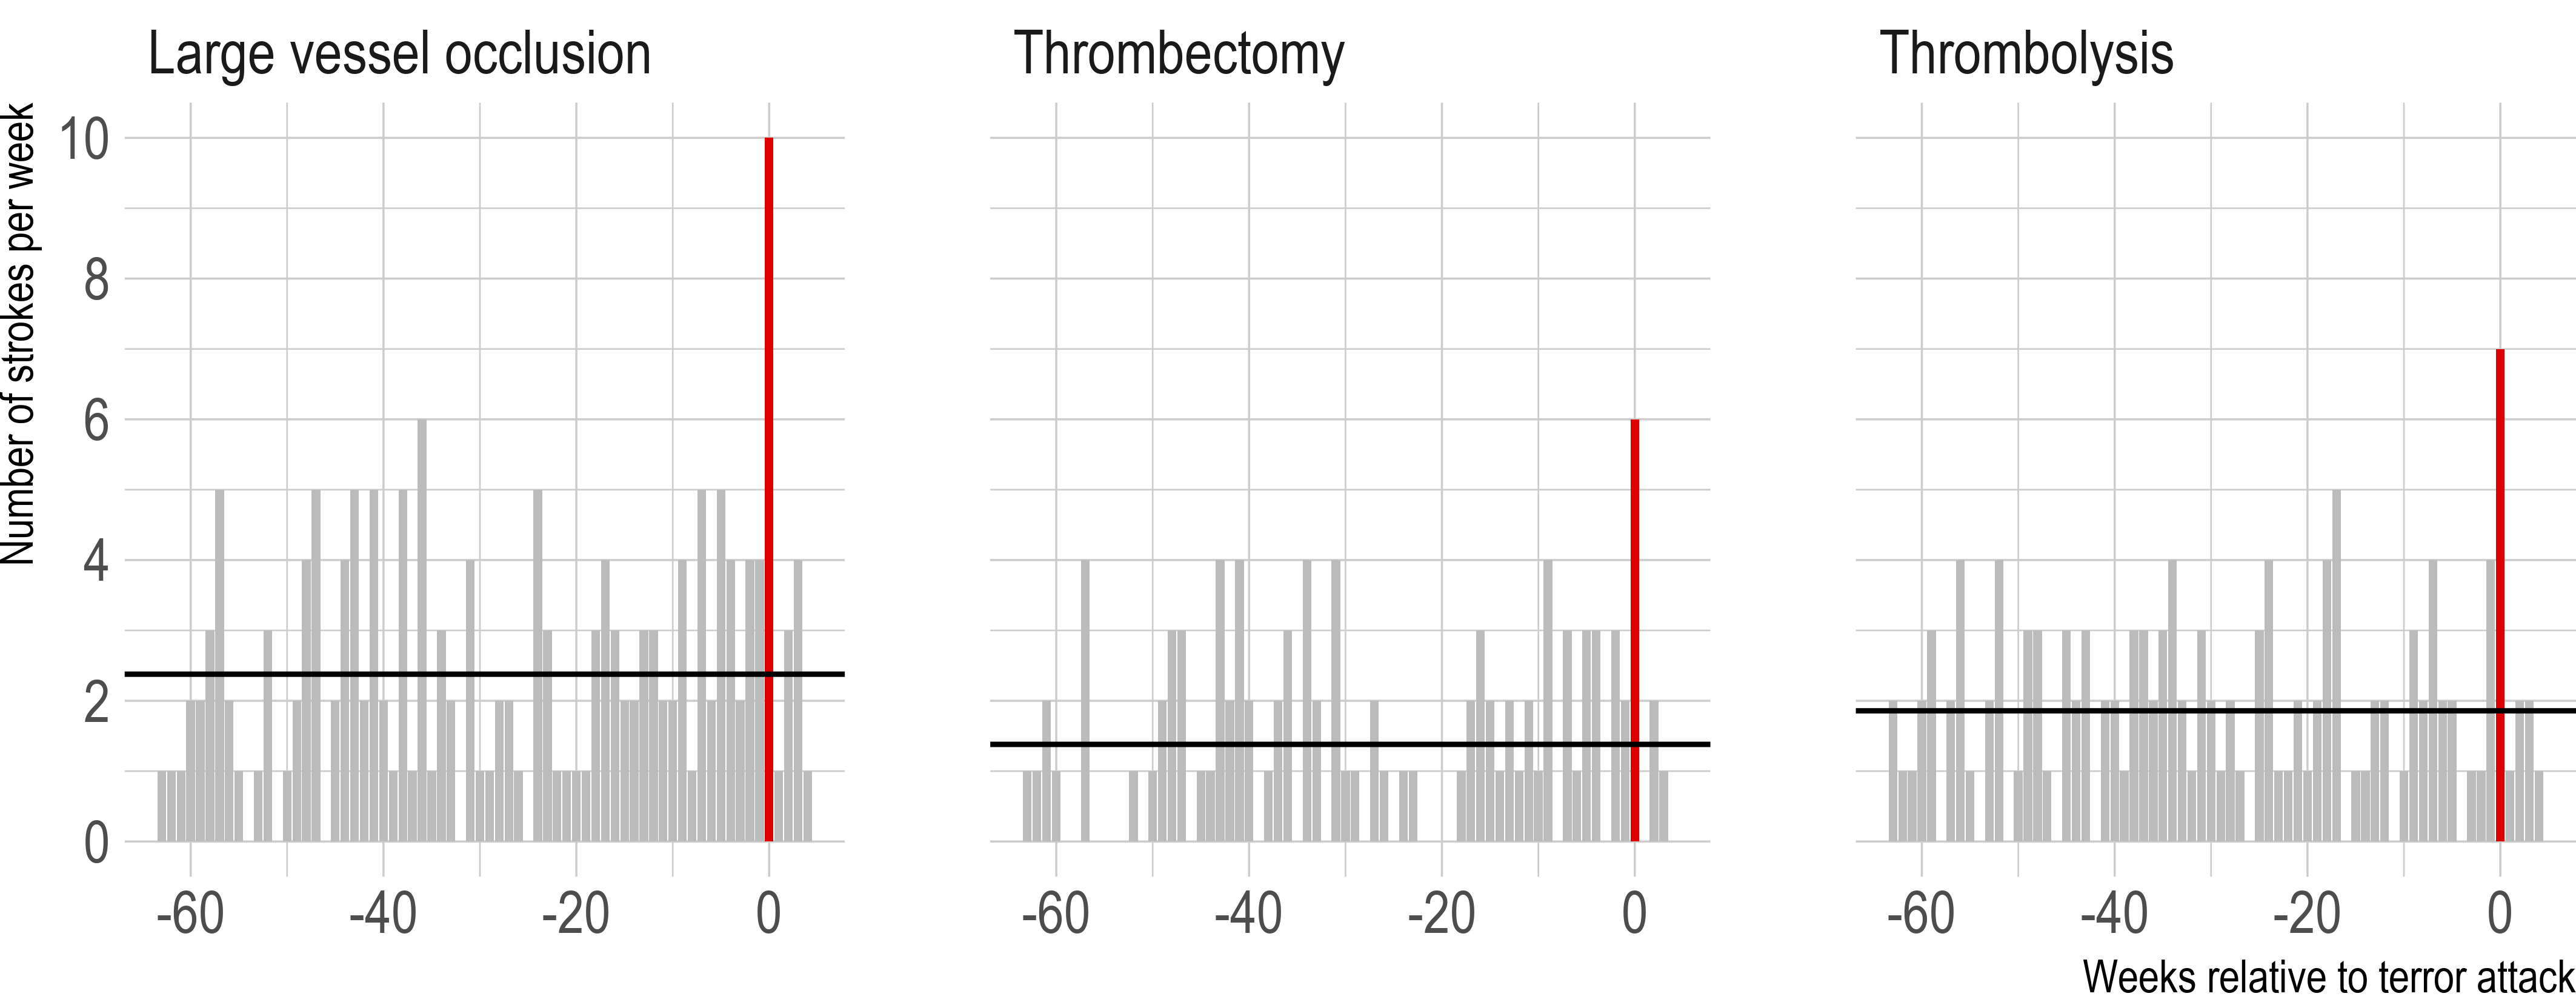
\includegraphics{Terror-attack-stroke_files/figure-latex/stroke-type-figure-1} \caption{Figure 2}\label{fig:stroke-type-figure}
\end{figure}

\hypertarget{supplementary-figure-caption}{%
\subsection{Supplementary Figure
Caption}\label{supplementary-figure-caption}}

Number of strokes per week by type at Christchurch Hospital, with the
week starting on Monday following the terror attack highlighted at week
0. The average number of strokes per week is shown by the black
horizontal line.

// Following plots are redundant

\hypertarget{references}{%
\section{References}\label{references}}

\end{document}
